\documentclass[11pt]{article}


%%% Packages
%%
\usepackage{amsmath}
\usepackage{amsfonts}
\usepackage{amssymb}
\usepackage{fancyhdr}
\usepackage{float}
\usepackage{graphicx}
\usepackage{listings}
\usepackage{pgfplots}
\usepackage{extramarks}
\usepackage{enumitem}
\usepackage{bm}
\usepackage{subcaption}
\usepackage{wasysym}
\usepackage[margin = 1in, headheight = 13.6pt]{geometry}
\usepackage[linktoc=all]{hyperref}
%%
%%%


%%% Formatting
%%
\parindent 0em
\parskip 1em
\pgfplotsset{compat=1.16}
\pagestyle{fancy}
\fancyhead{}
\fancyfoot{}
\fancyhead[L]{\slshape\MakeUppercase{{\myTitle}}}
\fancyhead[R]{\slshape{\myName}}
\fancyfoot[C]{\thepage}
%%
%%%


%%% User defined variables
%%
\def \myTitle {ECE301 Programming Assignment}
\def \myName {Elias Talcott}
\def \myDate {April 27, 2020}
%%
%%%


%%% Create Problem Sections
%%

\newcommand{\enterProblemHeader}[1]{
    \nobreak\extramarks{}{Problem \arabic{#1} continued on next page\ldots}\nobreak{}
    \nobreak\extramarks{Problem \arabic{#1} (continued)}{Problem \arabic{#1} continued on next page\ldots}\nobreak{}
}

\newcommand{\exitProblemHeader}[1]{
    \nobreak\extramarks{Problem \arabic{#1} (continued)}{Problem \arabic{#1} continued on next page\ldots}\nobreak{}
    \stepcounter{#1}
    \nobreak\extramarks{Problem \arabic{#1}}{}\nobreak{}
}

\setcounter{secnumdepth}{0}
\newcounter{partCounter}
\newcounter{homeworkProblemCounter}
\setcounter{homeworkProblemCounter}{1}
\nobreak\extramarks{Problem \arabic{homeworkProblemCounter}}{}\nobreak{}

%
% Homework Problem Environment
%
% This environment takes an optional argument. When given, it will adjust the
% problem counter. This is useful for when the problems given for your
% assignment aren't sequential. See the last 3 problems of this template for an
% example.
%
\newenvironment{homeworkProblem}[1][-1]{
    \ifnum#1>0
        \setcounter{homeworkProblemCounter}{#1}
    \fi
    \section{Problem \arabic{homeworkProblemCounter}}
    \setcounter{partCounter}{1}
    \enterProblemHeader{homeworkProblemCounter}
}{
    \exitProblemHeader{homeworkProblemCounter}
}


\begin{document}

\begin{titlepage}
\title{\myTitle}
\author{\myName}
\date{\myDate}
\maketitle
\vspace{1in}
\tableofcontents
\thispagestyle{empty}
\end{titlepage}

% Problem 1
\begin{homeworkProblem}

Develop a MATLAB program to graphically represent the convolution of two functions f(t) and g(t), where either function is a rectangular pulse of different lengths. Plot the following:
\begin{itemize}
\item The function f(t)
\item An animation of f(t) overlapping with g(t)
\item An animation of the convolution product which is only defined in the overlapping regions
\end{itemize}

\textbf{Solution}

% 5 screenshots of animation
\begin{figure}[h!]
	\begin{subfigure}[t]{0.45\linewidth}
		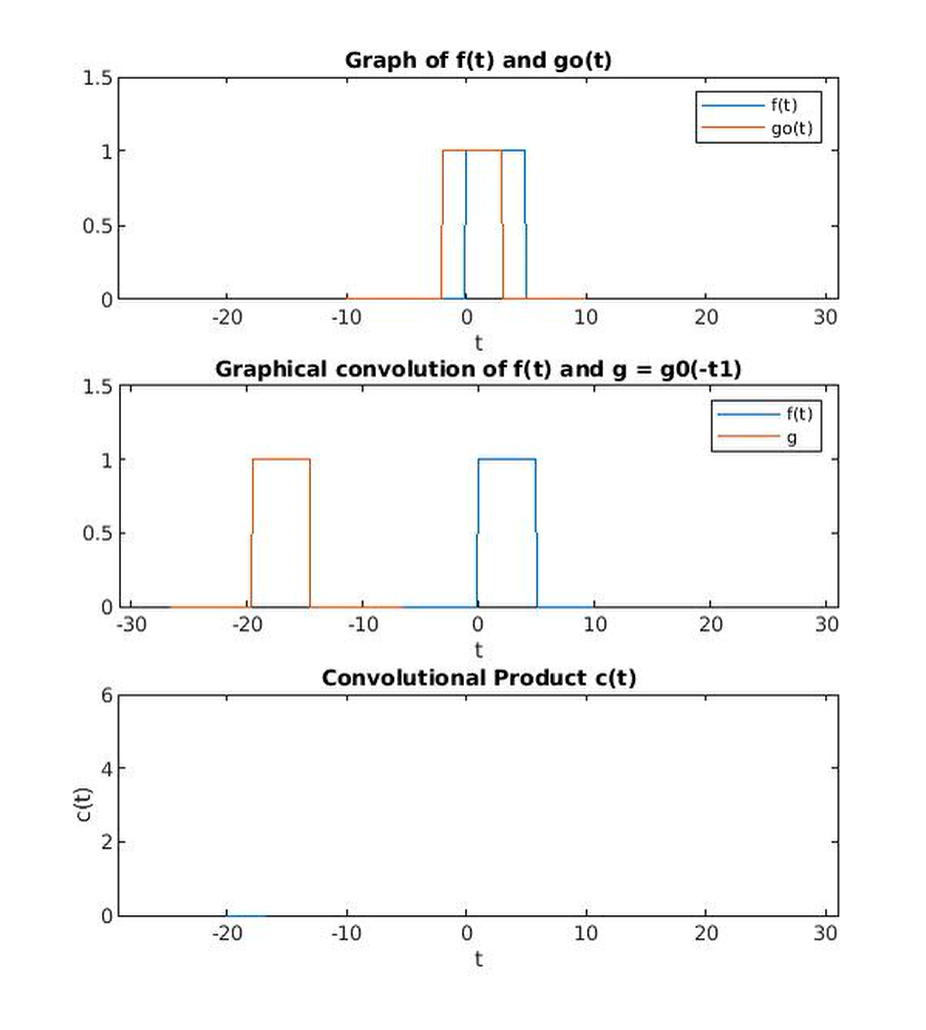
\includegraphics[width=\linewidth]{../Images/GraphicalConvolution_1.png}
	\end{subfigure}
	\begin{subfigure}[t]{0.45\linewidth}
		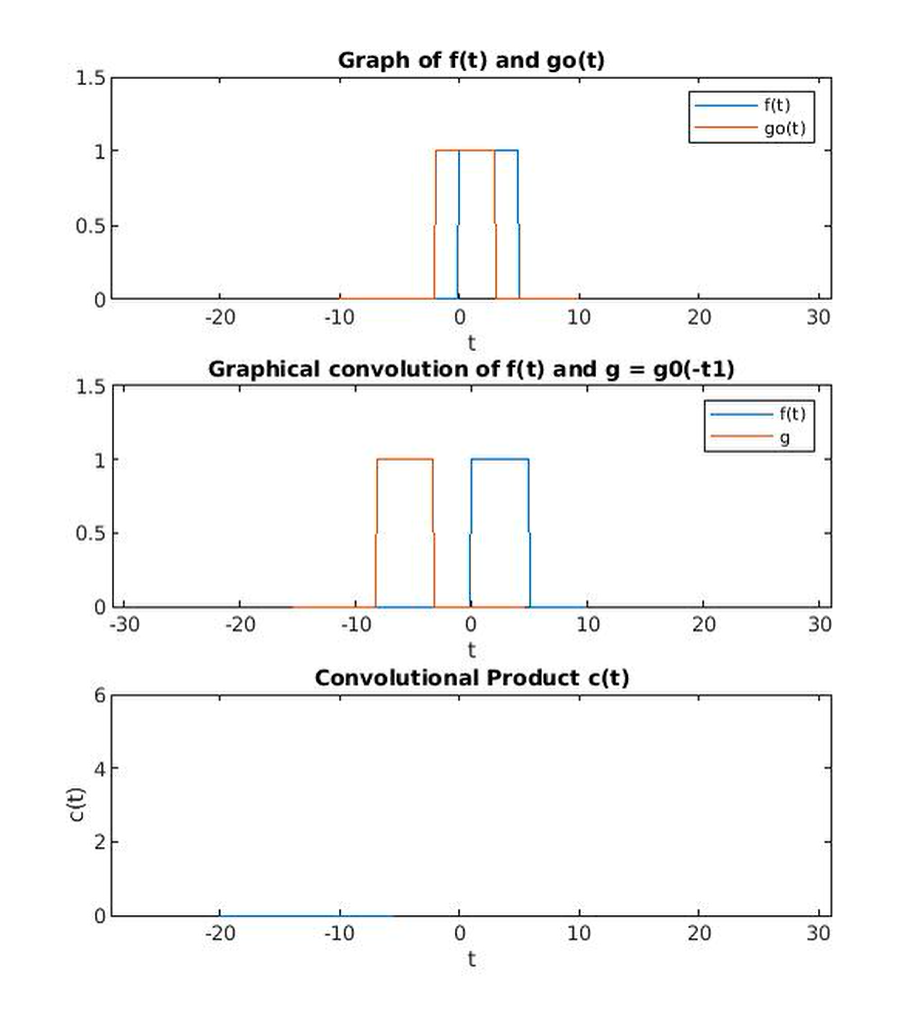
\includegraphics[width=\linewidth]{../Images/GraphicalConvolution_2.png}
	\end{subfigure}
\end{figure}
\pagebreak
\begin{figure}[h!]
	\begin{subfigure}[t]{0.45\linewidth}
		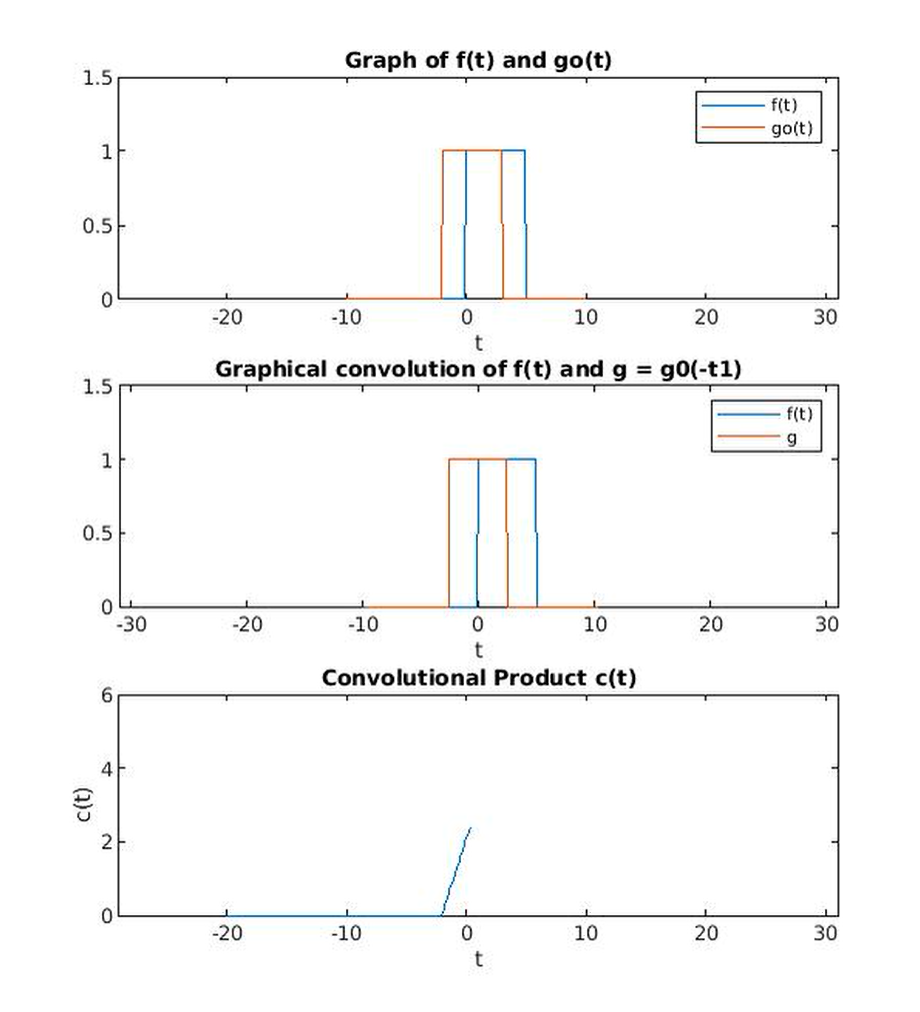
\includegraphics[width=\linewidth]{../Images/GraphicalConvolution_3.png}
	\end{subfigure}
	\begin{subfigure}[t]{0.45\linewidth}
		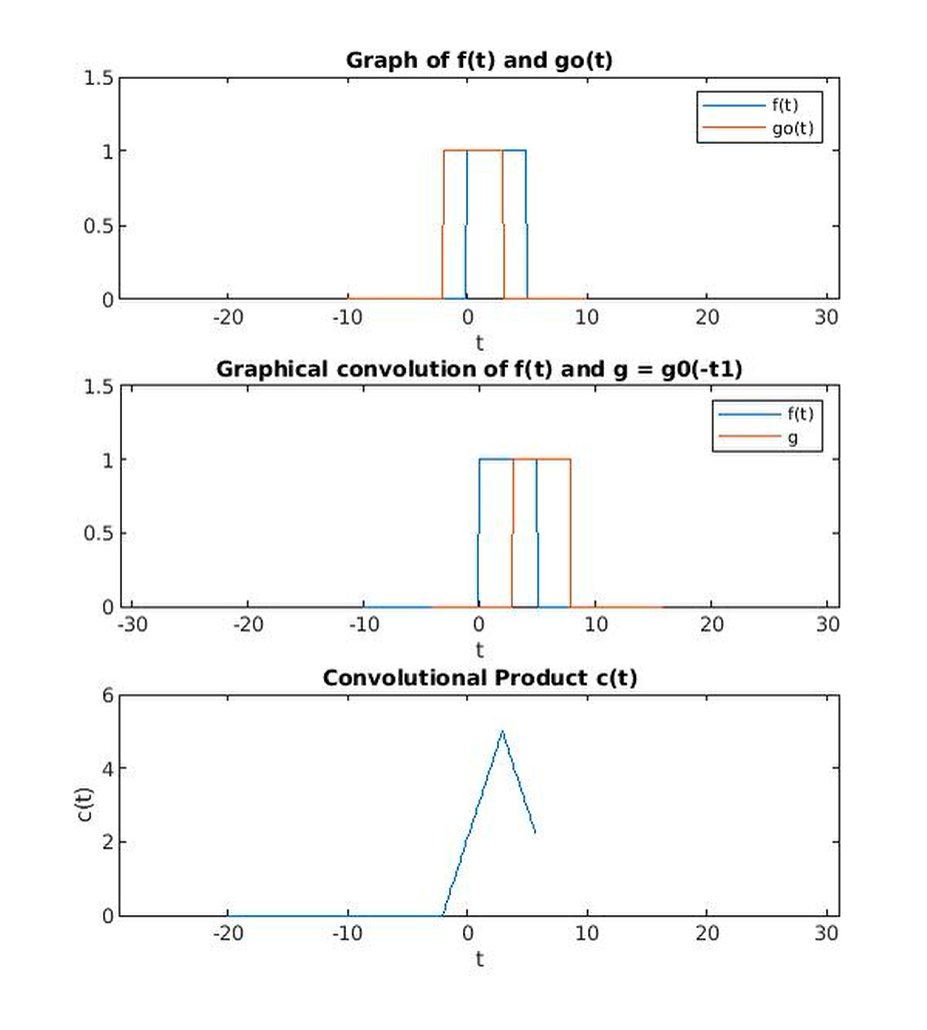
\includegraphics[width=\linewidth]{../Images/GraphicalConvolution_4.png}
	\end{subfigure}
\vspace{-5mm}
\end{figure}
\begin{figure}[h!]
	\begin{subfigure}[t]{0.45\linewidth}
		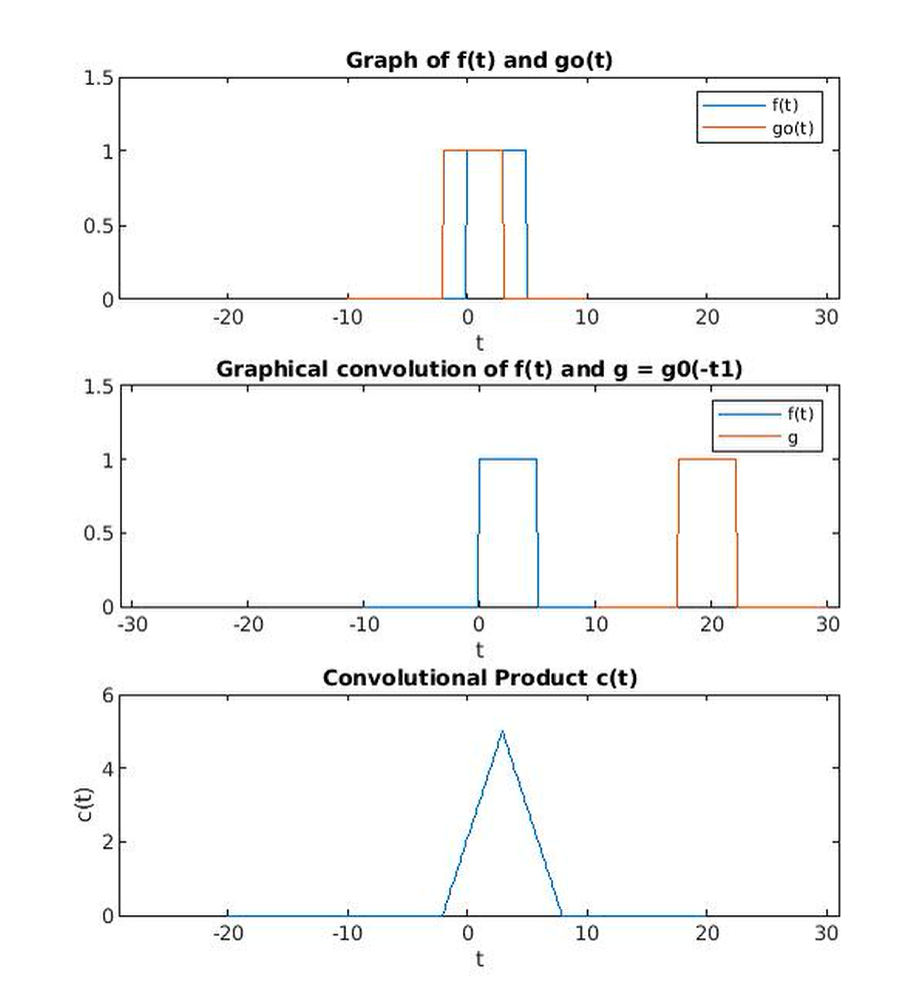
\includegraphics[width=\linewidth]{../Images/GraphicalConvolution_5.png}
	\end{subfigure}
\end{figure}

\vspace{-5mm}

% Explanation of solution
Graphical convolution involves passing one function through another and observing their overlap in each case. In this problem, there are 5 cases to consider:
\begin{itemize}
\item No overlap
\item Partial overlap
\item Full overlap
\item Partial overlap
\item No overlap
\end{itemize}
These cases are all observed in the second subplot as the function g passes through the function f ,and the convolution product c(t) in each case is calculated in the third subplot of each image.

\end{homeworkProblem}

\pagebreak

% Problem 2
\begin{homeworkProblem}

Represent the time domain signal in the figure below using its Fourier series coefficients. Plot this representation using 3, 5, and 10 sinusoidal terms. 

\begin{figure}[h!]
	\begin{center}
	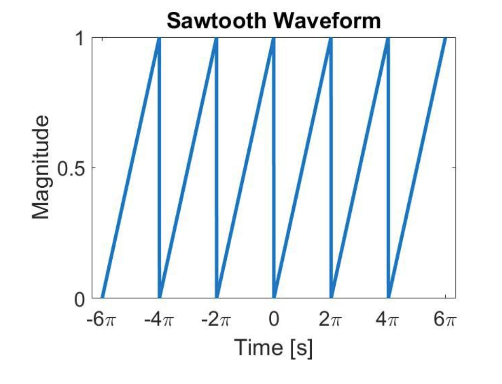
\includegraphics[width=0.5\linewidth]{../Images/Problem2.png}	
	\end{center}
\end{figure}

\vspace{-5mm}

\textbf{Solution}

% Expression for signal in terms of sines and cosines
Using the MATLAB curve fitting tool (cftool), I found the Fourier series representation of the signal f(t) to be $f(t) = 0.5 - \sum\limits_{k=1}^{k=\infty} \frac{1}{k\pi} \sin(kt)$. This was supported by my own derivation of $D_k$, in which I came to the result $D_k = \frac{j}{2\pi k}$. The Fourier series has no cosine terms since it is representing an odd function.

\[
	\begin{split}
	T &= 2\pi \textrm{, } \omega_0 = 1
	\\	
	D_k &= \int\limits_{t = 0}^{t = 2\pi} \frac{t}{2\pi} e^{-jkt} \frac{dt}{2\pi}
	\\
	D_k &= \frac{1}{4\pi^2} \int\limits_{t = 0}^{t = 2\pi} te^{-jkt}\; dt
	\\
	D_k &= \frac{1}{4\pi^2} \left[e^{-jkt}\left(\frac{jt}{k} + \frac{1}{k^2} \right) \right]_{t = 0}^{t = 2\pi}  
	\\
	D_k &= \frac{jk2\pi e^{-jk2\pi} + e^{-jk2\pi} - 1}{4\pi^2k^2}
	\\
	D_k &= \frac{jk2\pi\cos(2\pi k) + \cos(2\pi k) - k2\pi\sin(2\pi k) + j\sin(2\pi k) - 1}{4\pi^2k^2}
	\\
	\sin(2\pi k) &= 0 \textrm{ for all integers } k
	\\
	\cos(2\pi k) &= 1 \textrm{ for all integers } k
	\\
	\therefore D_k &= \frac{j}{2\pi k}
	\end{split}
\]

\pagebreak

% Three plots of signal
\begin{figure}[h!]
	\begin{center}
	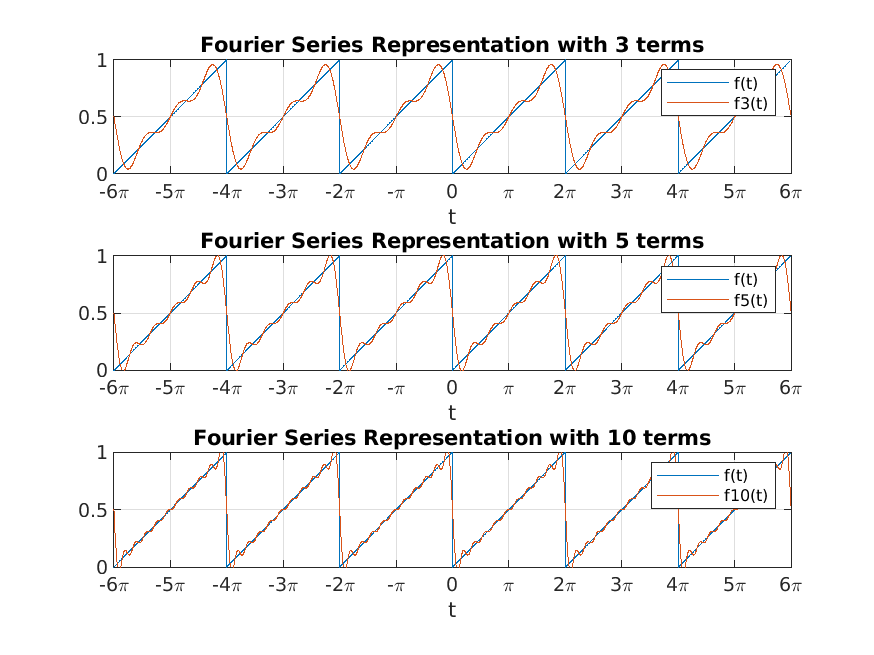
\includegraphics[width=0.8\linewidth]{../Images/Sawtooth.png}
	\end{center}
\end{figure}

% Explanation of plots
As the three subplots above demonstrate, using more and more terms creates a closer approximation to the actual signal. As the number of terms approaches infinity, the Fourier series representation becomes identical to the actual signal.


\end{homeworkProblem}

\pagebreak

% Problem 3
\begin{homeworkProblem}

Plot the output signal given the RC circuit and input signal in the figure below. Take the time period of the signal to be unity and $R=10k\Omega$, $C=5\mu F$.

\begin{figure}[h!]
	\begin{center}
	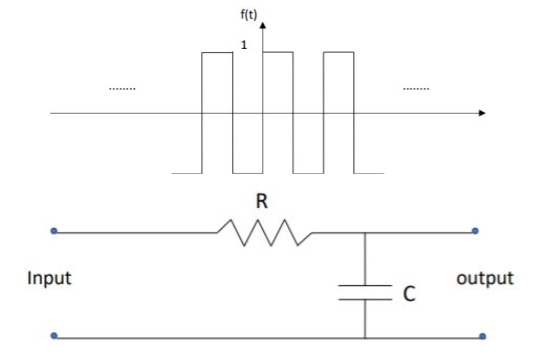
\includegraphics[width=0.5\linewidth]{../Images/Problem3.png}
	\end{center}
\end{figure}

\textbf{Solution}

\begin{figure}[h!]
	\begin{subfigure}[t]{0.45\linewidth}
		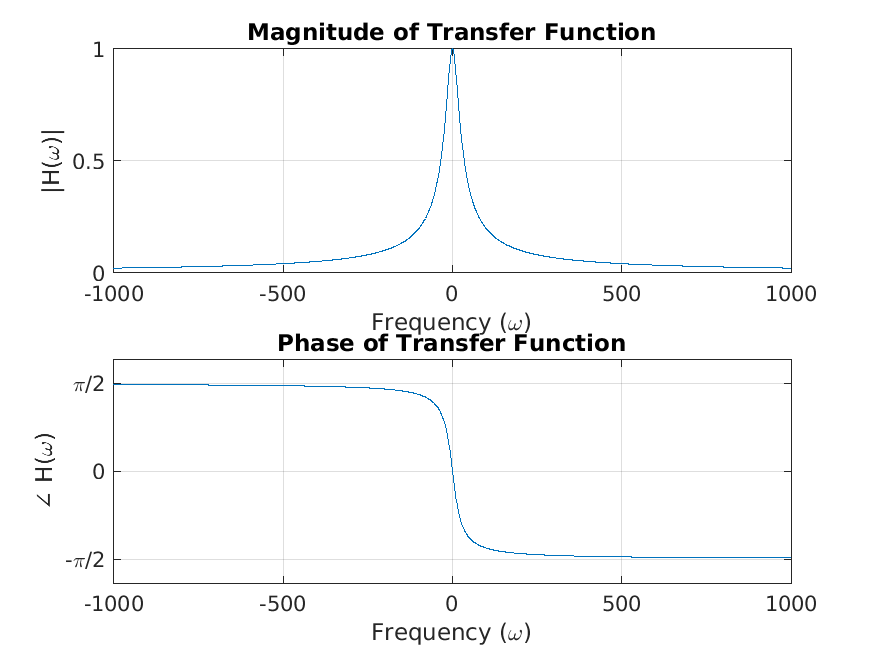
\includegraphics[width=\linewidth]{../Images/TransferFunction.png}
	\end{subfigure}
	\begin{subfigure}[t]{0.45\linewidth}
		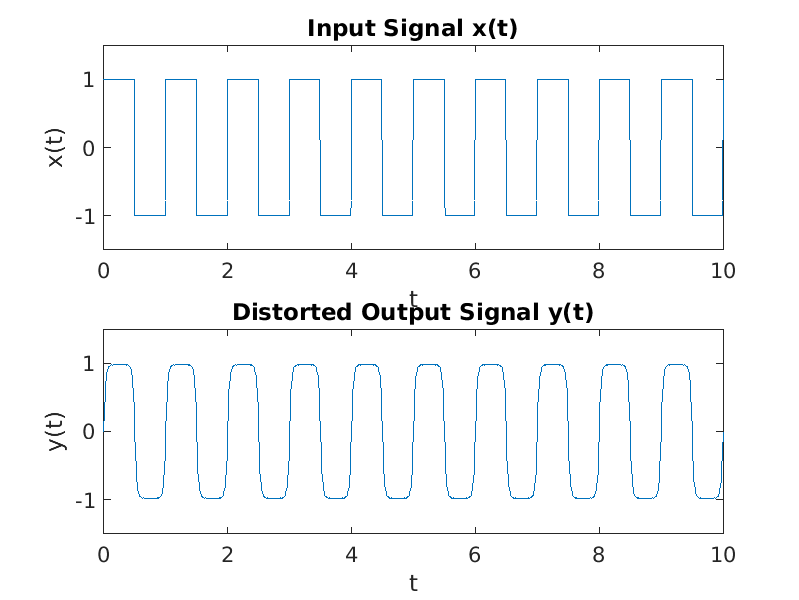
\includegraphics[width=\linewidth]{../Images/OutputSignal.png}
	\end{subfigure}
\end{figure}


I found the transfer function of the RC circuit to be $H(\omega) = \frac{1}{1 + j0.05\omega}$. The magnitude and phase of this transfer function are shown in the figure on the left above. I used this transfer function and the Fourier series coefficients of the input waveform to calculate the output waveform, which is shown in the figure on the right above. The input signal is shown in the first subplot and the distorted output signal is shown in the second subplot. 


\end{homeworkProblem}

\pagebreak

% Problem 4
\begin{homeworkProblem}

Plot the frequency domain spectral representation of the signal $f(t) = e^{-at^2}$ for $a=1,10,100$.

\textbf{Solution}

\begin{figure}[h!]
	\begin{center}
	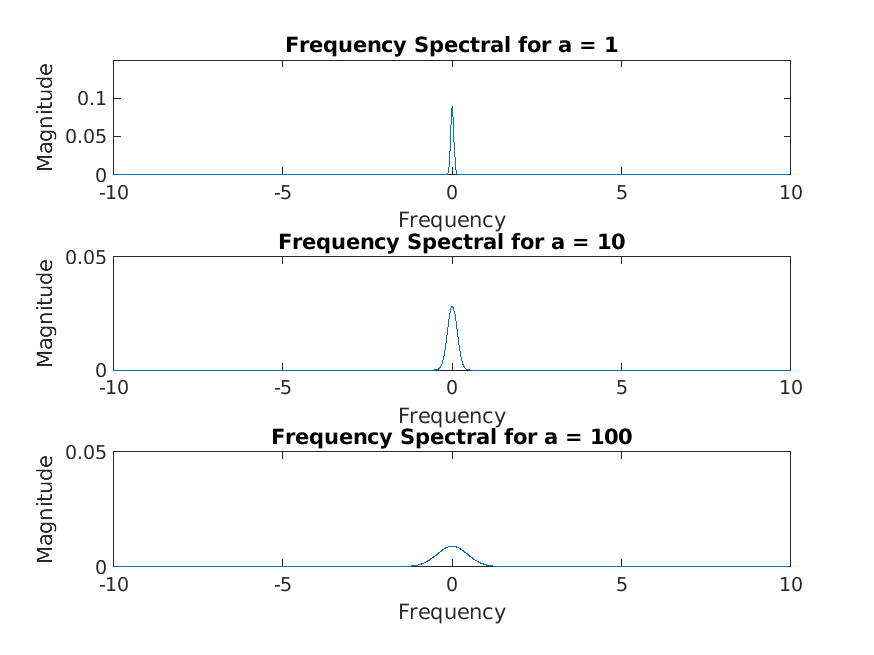
\includegraphics[width=0.7\linewidth]{../Images/Spectrals.png}
	\end{center}
\end{figure}

In order to find the Fourier transform of each signal f(t), I used the MATLAB function fft. For each function f with a different value of a, I called abs(fftshift(fft(f))) in order to arrive at the results in the figure above. These figures demonstrate the relationship between signals in the time domain and in the frequency domain. As the signal contracted in the time domain, it simultaneously expanded in the frequency domain.

\end{homeworkProblem}

\pagebreak

% Problem 5
\begin{homeworkProblem}

Plot and explain your observations of a rotating spot inside a circle for the following conditions:
\begin{enumerate}[label=(\alph*)]
\item Nyquist frequency \textgreater\textgreater\; Signal frequency
\item Nyquist frequency \textgreater\; Signal frequency
\item Nyquist frequency = Signal frequency
\item Nyquist frequency \textless\; Signal frequency
\item Nyquist frequency = 0.5 * Signal frequency
\item Nyquist frequency \textless\; 0.5 * Signal frequency
\end{enumerate}

\textbf{Solution}

\captionsetup[subfigure]{labelformat=empty}

\begin{figure}[h!]
	\begin{subfigure}[t]{0.45\linewidth}
		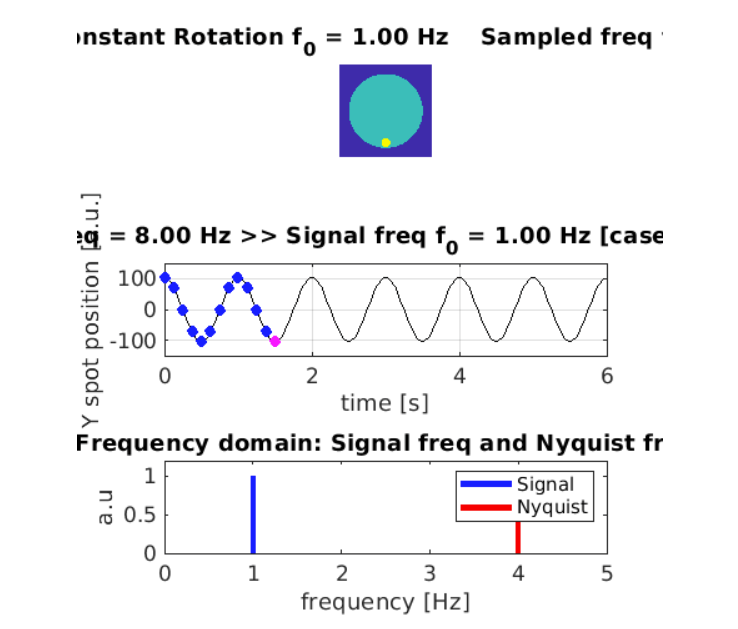
\includegraphics[width=\linewidth]{../Images/Sample_1.png}
		\caption{(a) Nyquist frequency \textgreater\textgreater\; Signal frequency}
	\end{subfigure}
	\begin{subfigure}[t]{0.45\linewidth}
		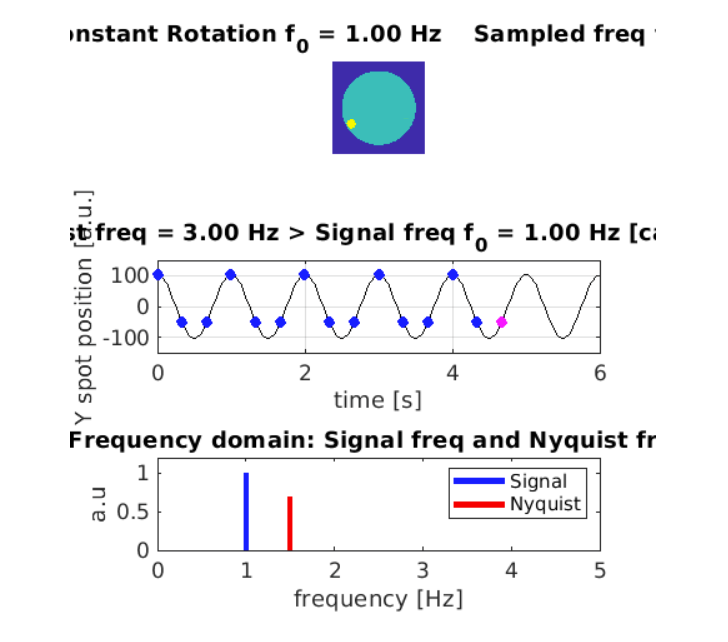
\includegraphics[width=\linewidth]{../Images/Sample_2.png}
		\caption{(b) Nyquist frequency \textgreater\; Signal frequency}
	\end{subfigure}
\end{figure}
\pagebreak
\begin{figure}[h!]
	\begin{subfigure}[t]{0.45\linewidth}
		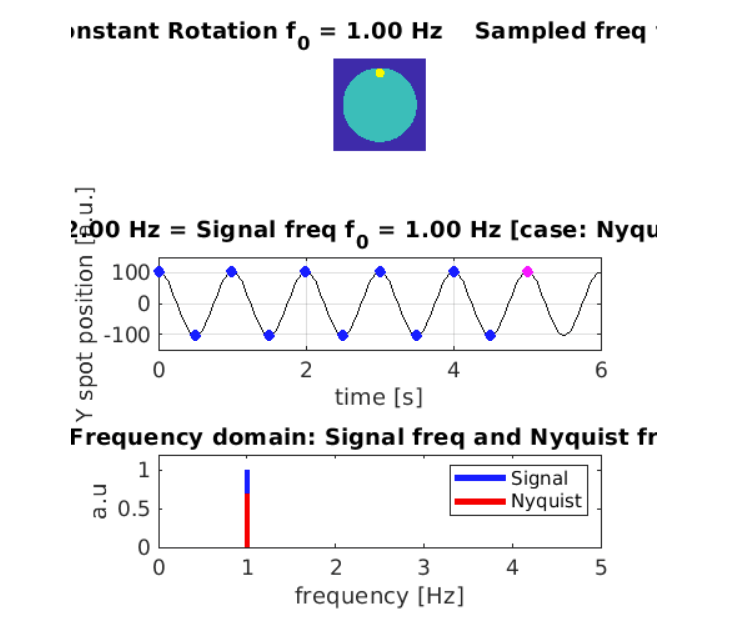
\includegraphics[width=\linewidth]{../Images/Sample_3.png}
		\caption{(c) Nyquist frequency = Signal frequency}
	\end{subfigure}
	\begin{subfigure}[t]{0.45\linewidth}
		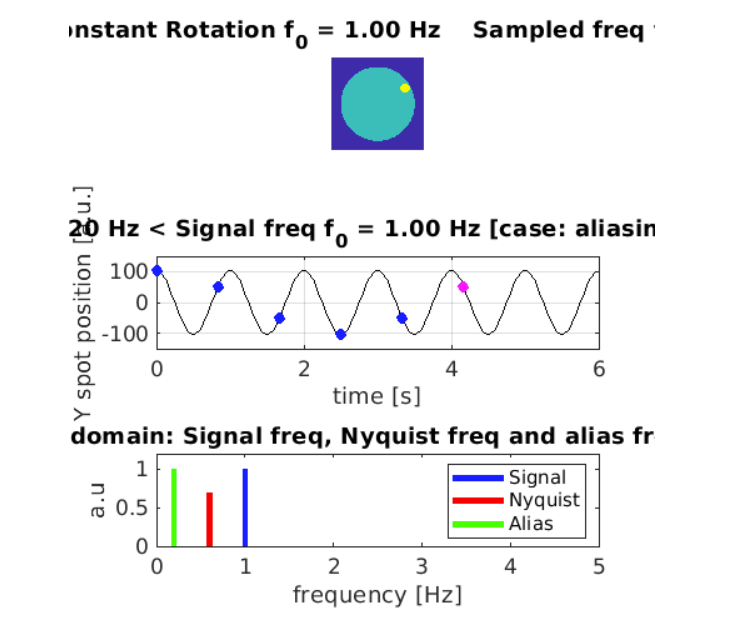
\includegraphics[width=\linewidth]{../Images/Sample_4.png}
		\caption{(d) Nyquist frequency \textless\; Signal frequency}
	\end{subfigure}
\end{figure}
\begin{figure}[h!]
	\begin{subfigure}[t]{0.45\linewidth}
		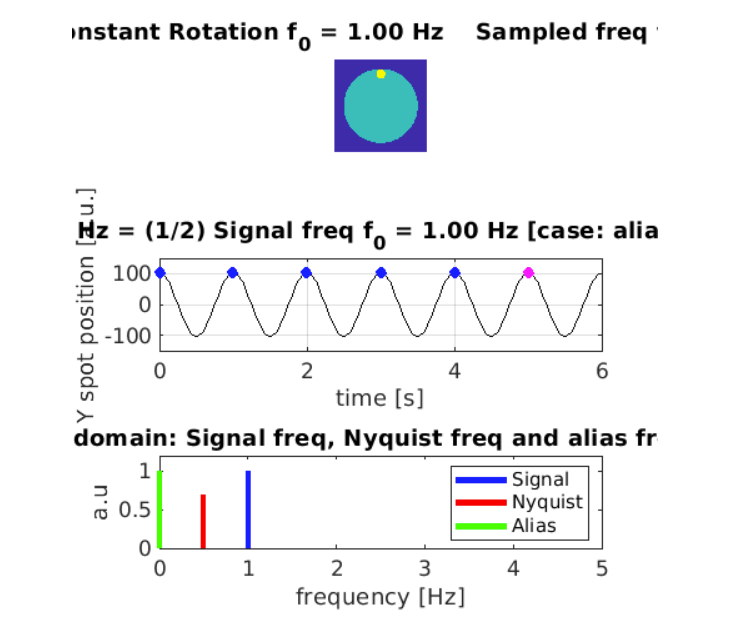
\includegraphics[width=\linewidth]{../Images/Sample_5.png}
		\caption{(e) Nyquist frequency = 0.5 * Signal frequency}
	\end{subfigure}
	\begin{subfigure}[t]{0.45\linewidth}
		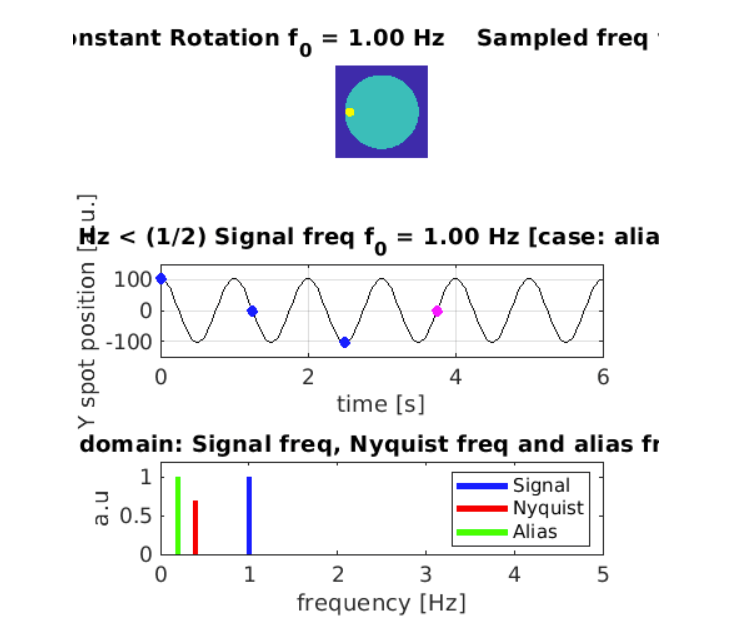
\includegraphics[width=\linewidth]{../Images/Sample_6.png}
		\caption{(f) Nyquist frequency \textless\; 0.5 * Signal frequency}
	\end{subfigure}
\end{figure}

\vspace{1cm}

My observations for each frequency relationship is as follows:

\begin{enumerate}[label=(\alph*)]
\item The spot appears to be moving smoothly in the clockwise direction
\item The spot appears to move in a choppy motion in the clockwise direction
\item The spot moves from top to bottom with no apparent direction
\item The spot appears to move in a choppy motion in the counterclockwise direction
\item The spot does not move at all from the top position
\item The spot appears to move in quarters in the clockwise direction
\end{enumerate}

\end{homeworkProblem}

\pagebreak

% Problem 6
\begin{homeworkProblem}

The song is "Never Gonna Give You Up" by Rick Astley.

I will \textbf{not} be Rick Rolled over and over again for this problem. ;)

\end{homeworkProblem}

\end{document}
